\section{Accurator framework}
\label{architecture}
Our main assumption is that personalizing the niche sourcing process increases the quality of annotations. We believe the we can use specific techniques to identify niches and create user profiles. Based on the user profiles we can recommend relevant tasks to the user and apply trust mechanisms to motivate users, provide feedback and improve the recommendations. In Figure 1 we show the interfaces of Accurator that map onto the the aforementioned challenges. 

\begin{figure*}[hbt]
	\centering
	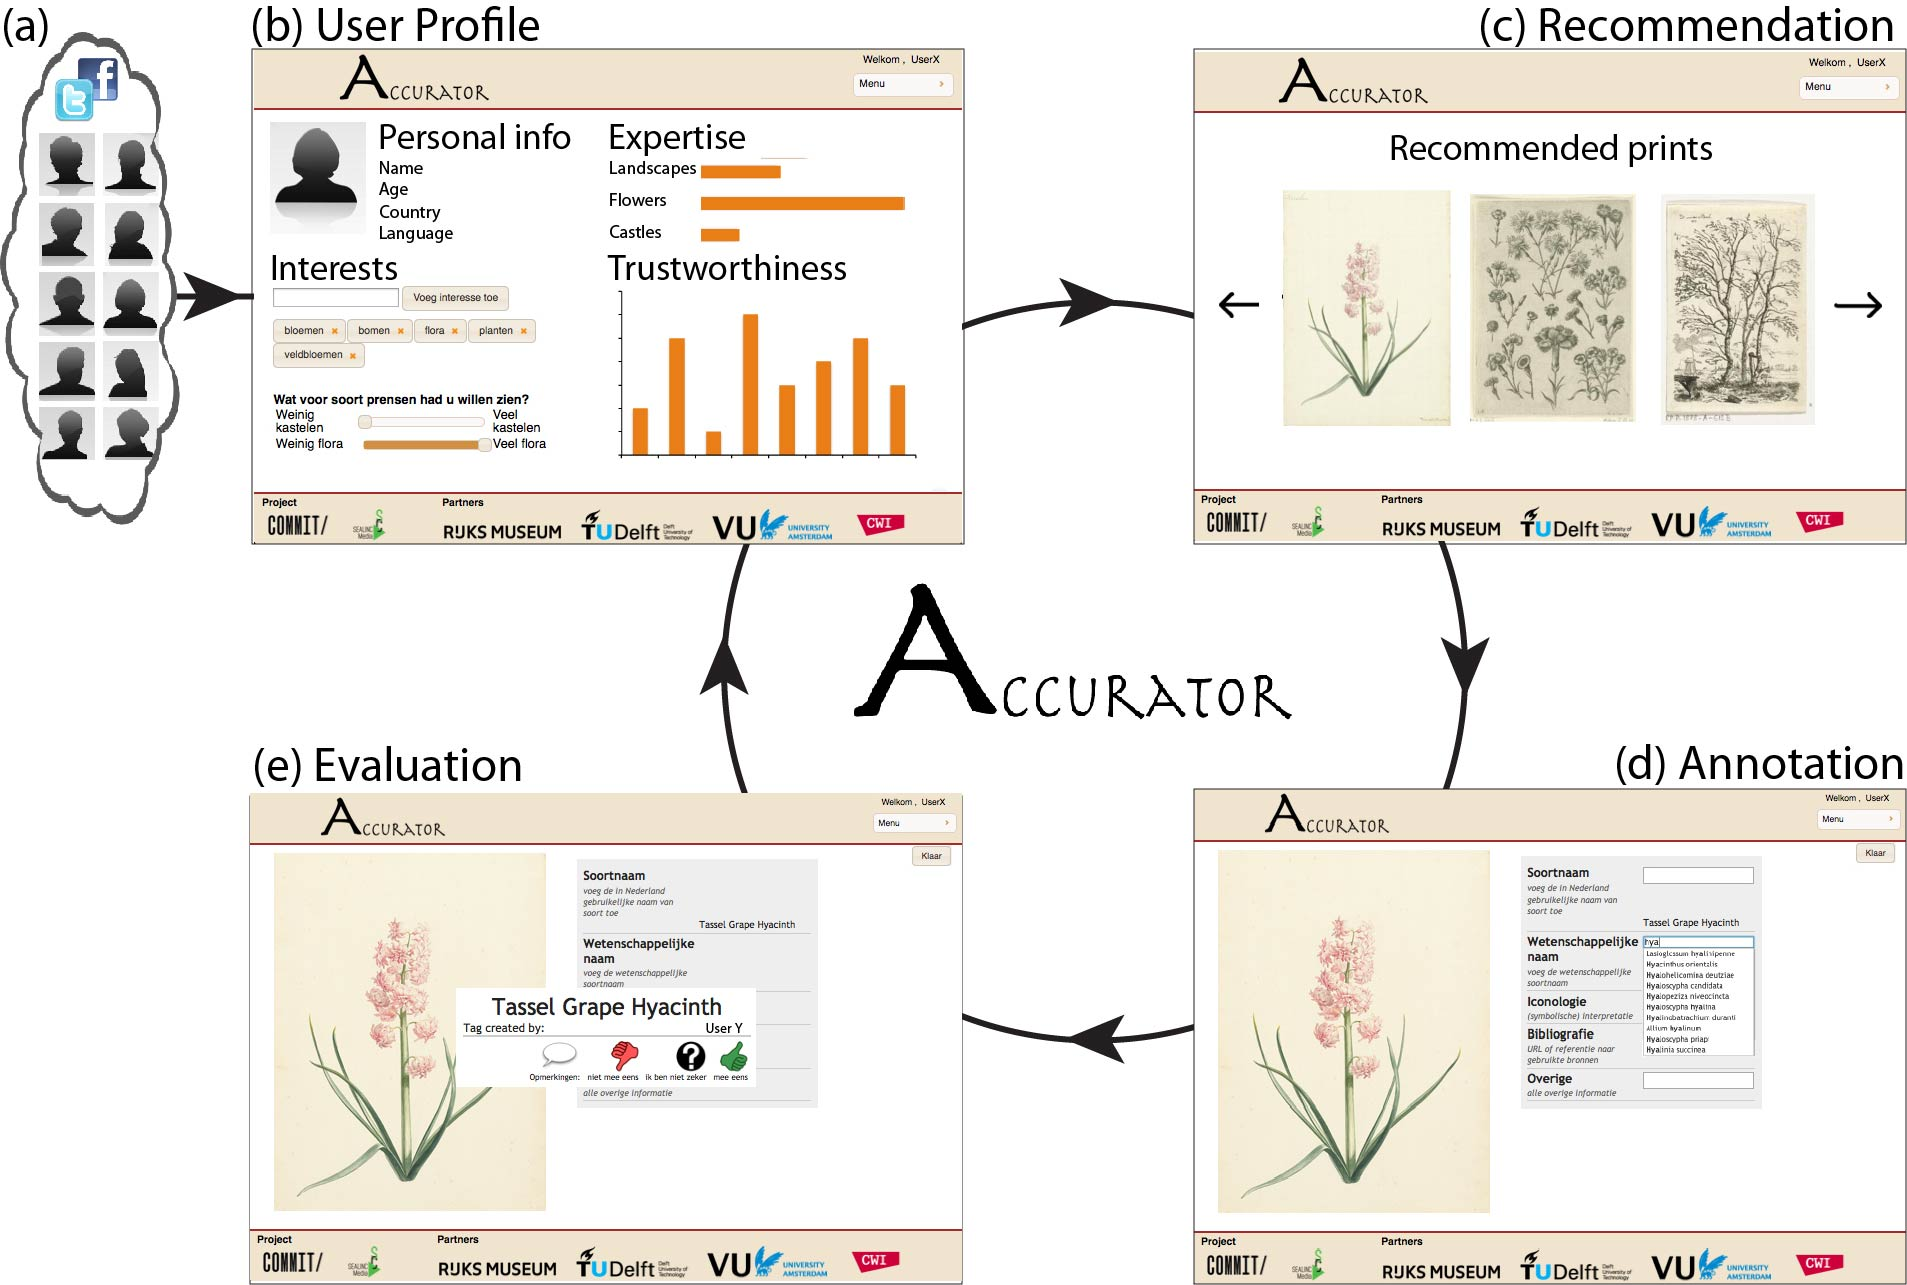
\includegraphics[width=\textwidth]{accurator_diagram.jpg}
  	\caption{Diagram}
\end{figure*}

The process starts, see Figure 1a, with searching the social web for user generated content that is relevant for a topic. We calculate the relevance of the content creators in respect to then topic and exploit social relations to identify a topical niche. We motivate the niche to use Accurator and when a person starts using Accurator a user profile, see Figure 1b, is build based on available data and shown to the user. The user can specify additional social web accounts.

Figure 1c shows the recommendation of tasks for a user. The recommendation strategy is based on specific patterns in the data, the user profile of the user and the current annotation quality of an item. Accurator allows to easily change between different strategies to cater for different users and a future task is to automatically adapt the choice of strategy based on that user profile. The choice of recommended item can affects the calculated interest of that user.

Figure 1d shows the interface where users add their annotations to a collection item. Choice of fields dependent on the topic and the expertise of the user on that topic. Users with more expertise on that topic are allowed to enter more difficult fields. Accurator can also be configured to use a vocabulary for a field to support the user. Figure 1e shows a similar interface where users review the annotations of other users. Reviewing tasks are only available to users who are trustworthy and have a certain level of expertise. The result of a review affects 1) the quality of an annotation, 2) the expertise level of a user and 3) the trustworthiness of a user.

Another aspect that holds for all interfaces is that they should be intuitive and helpful. Users who encounter difficulties with the interface will not return. 

Accurator is build using Cliopatria to store RDF, GWT for the user interface and GAE for hosting. Accurator is now used for experimentation with data from the Rijksmuseum in the Netherlands and a demo is available at \url{http://rma-accurator.appspot.com}.



